\chapter{Anexo}

\section{Esquemático Completo}

\begin{figure}[H]
	\centering
	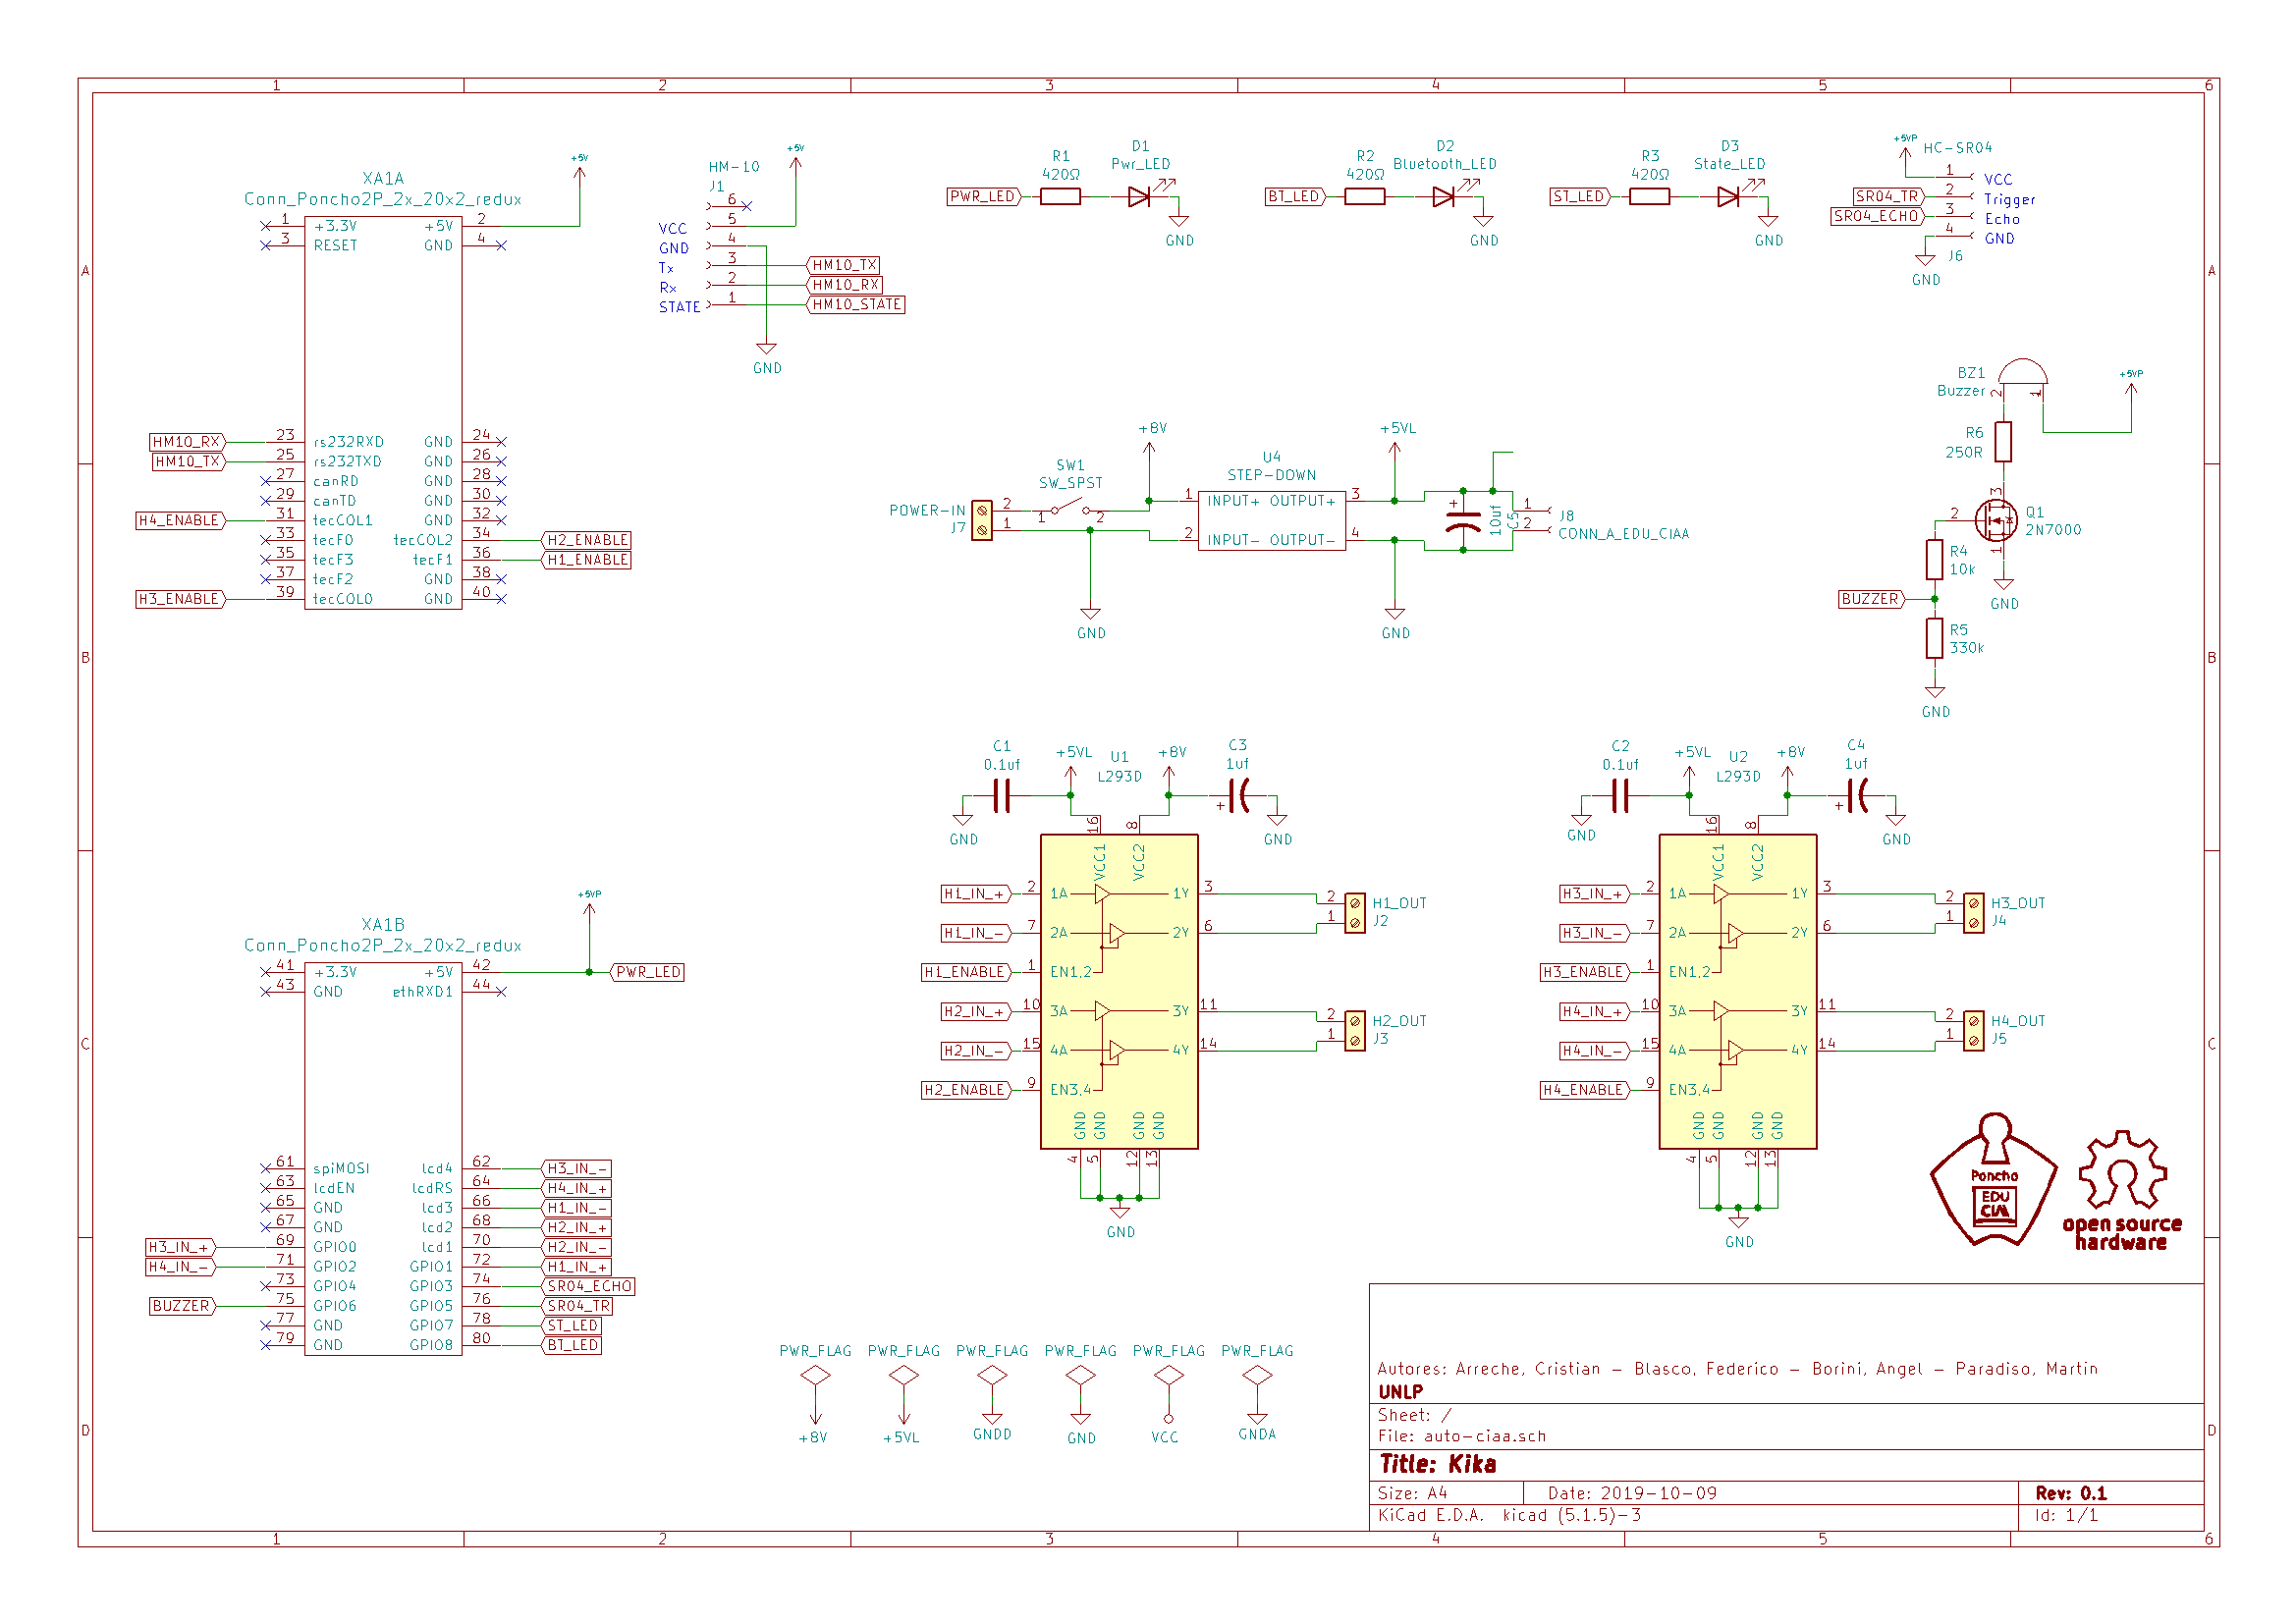
\includegraphics[width=0.85\textheight, angle=90]{informe_3/schem}
	\label{fig:schem}
\end{figure}

\section{Imágenes de Capas}

\begin{figure}[H]
	\centering
	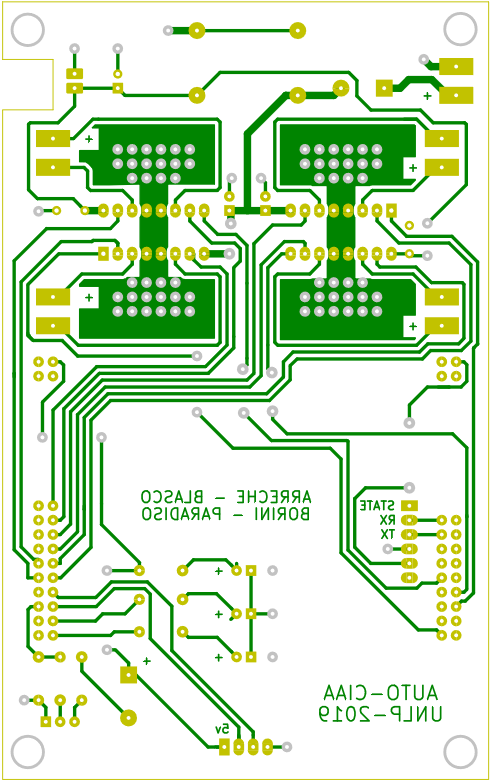
\includegraphics[height=0.8\linewidth, angle=-90]{informe_4/capa_bg.png}
	\label{fig:capa_bg}
	\caption{Capa de cobre inferior}
\end{figure}

\begin{figure}[H]
\centering
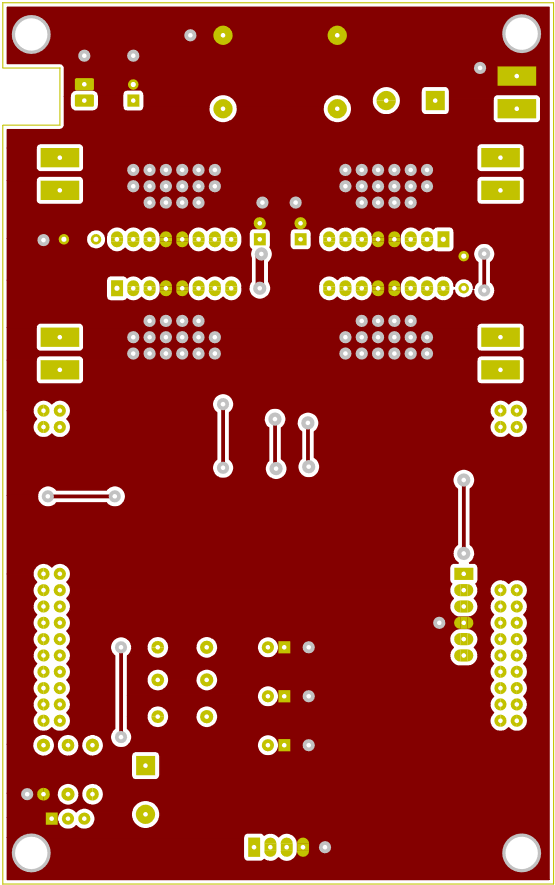
\includegraphics[height=0.8\linewidth, angle=-90]{informe_4/capa_fg.png}
\label{fig:capa_fg}
\caption{Capa de cobre superior (con plano de tierra)}
\end{figure}

\begin{figure}[H]
	\centering
	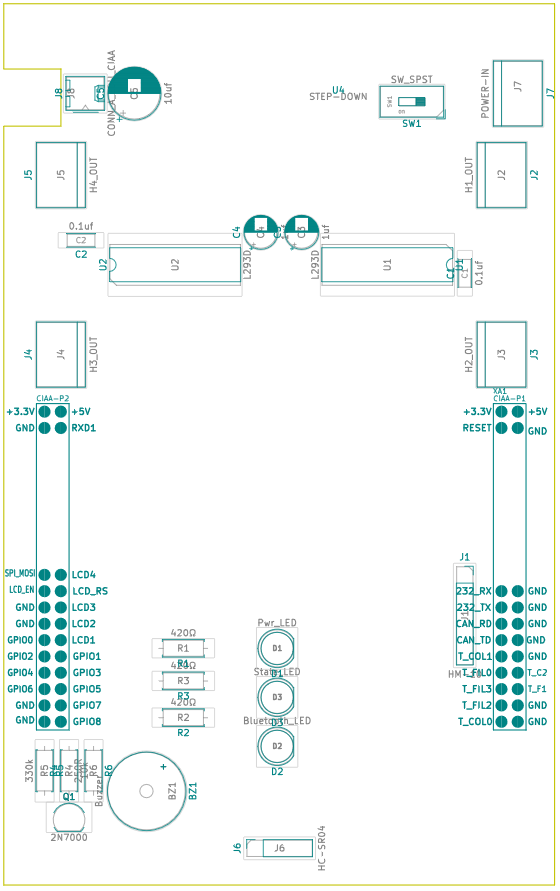
\includegraphics[height=0.8\linewidth, angle=-90]{informe_4/capa_comp.png}
	\label{fig:capa_comp}
	\caption{Componentes}
\end{figure}

\section{Imágenes en 3D}

\begin{figure}[H]
	\centering
	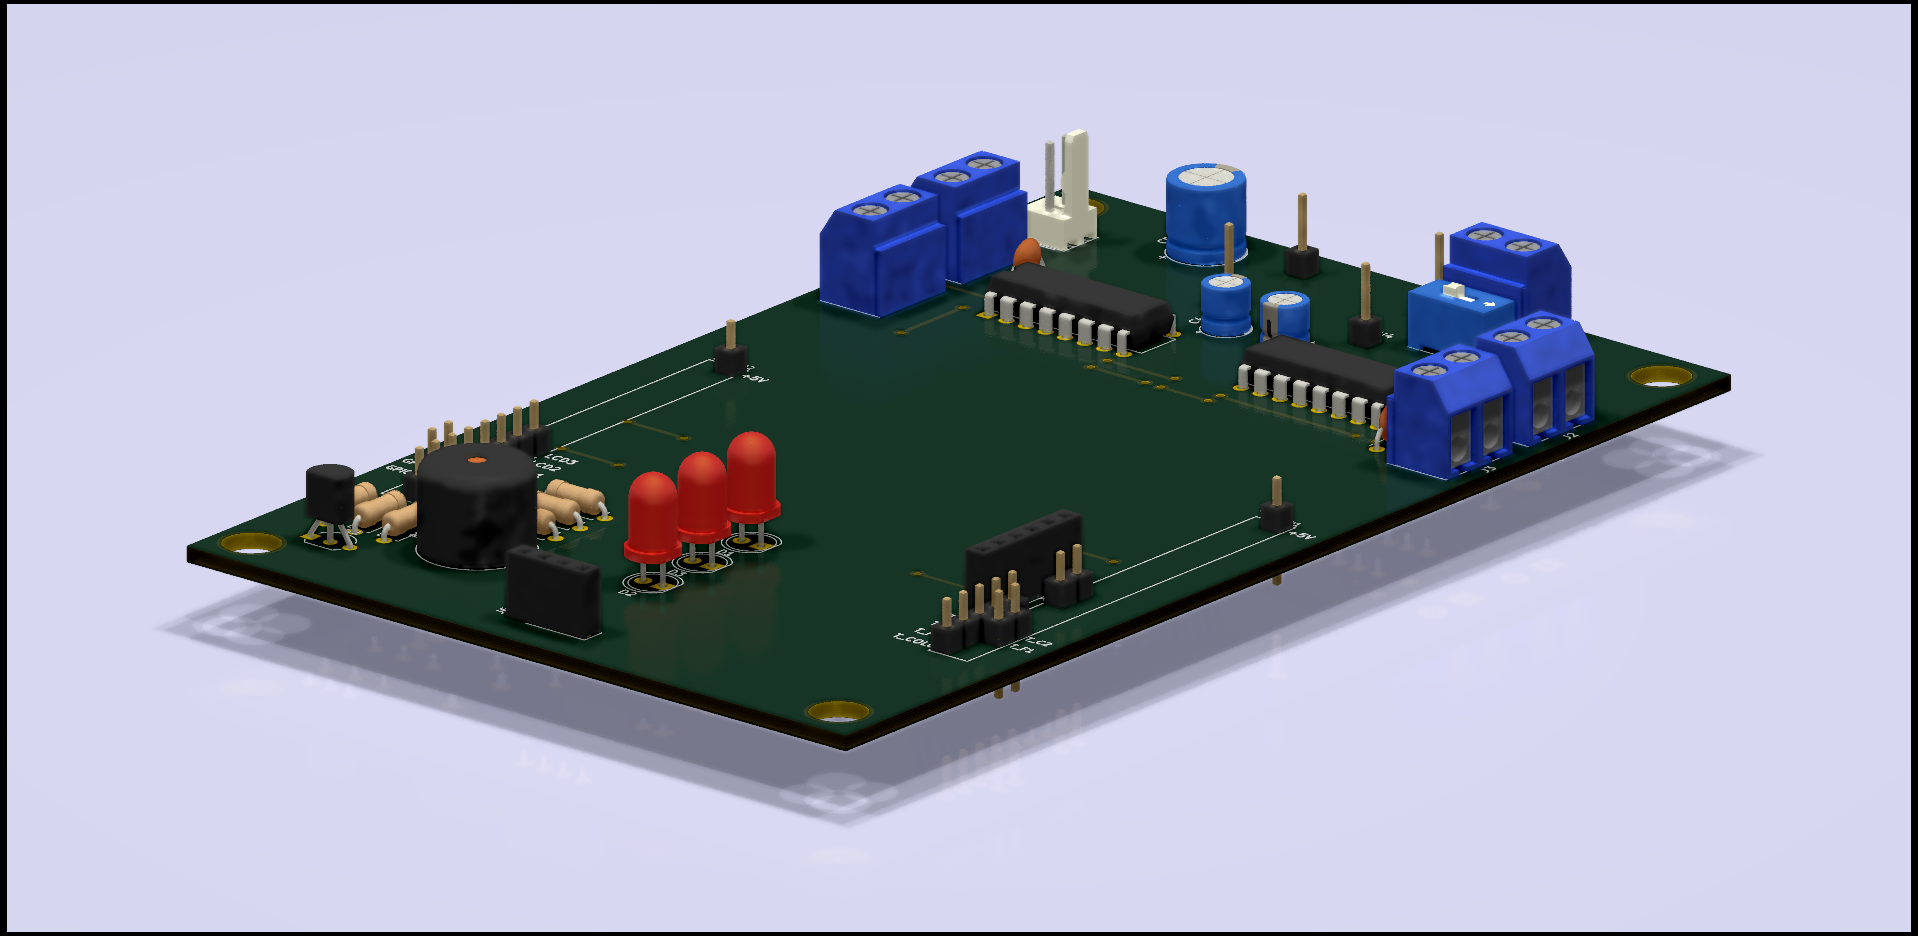
\includegraphics[width=0.8\linewidth]{informe_3/vista_iso.png}
	\caption{Vista isométrica generada con KiCad}
	\label{fig:3d}
\end{figure}

\begin{figure}[H]
	\centering
	\begin{tabular}{cc}
		\subfloat[Frontal]{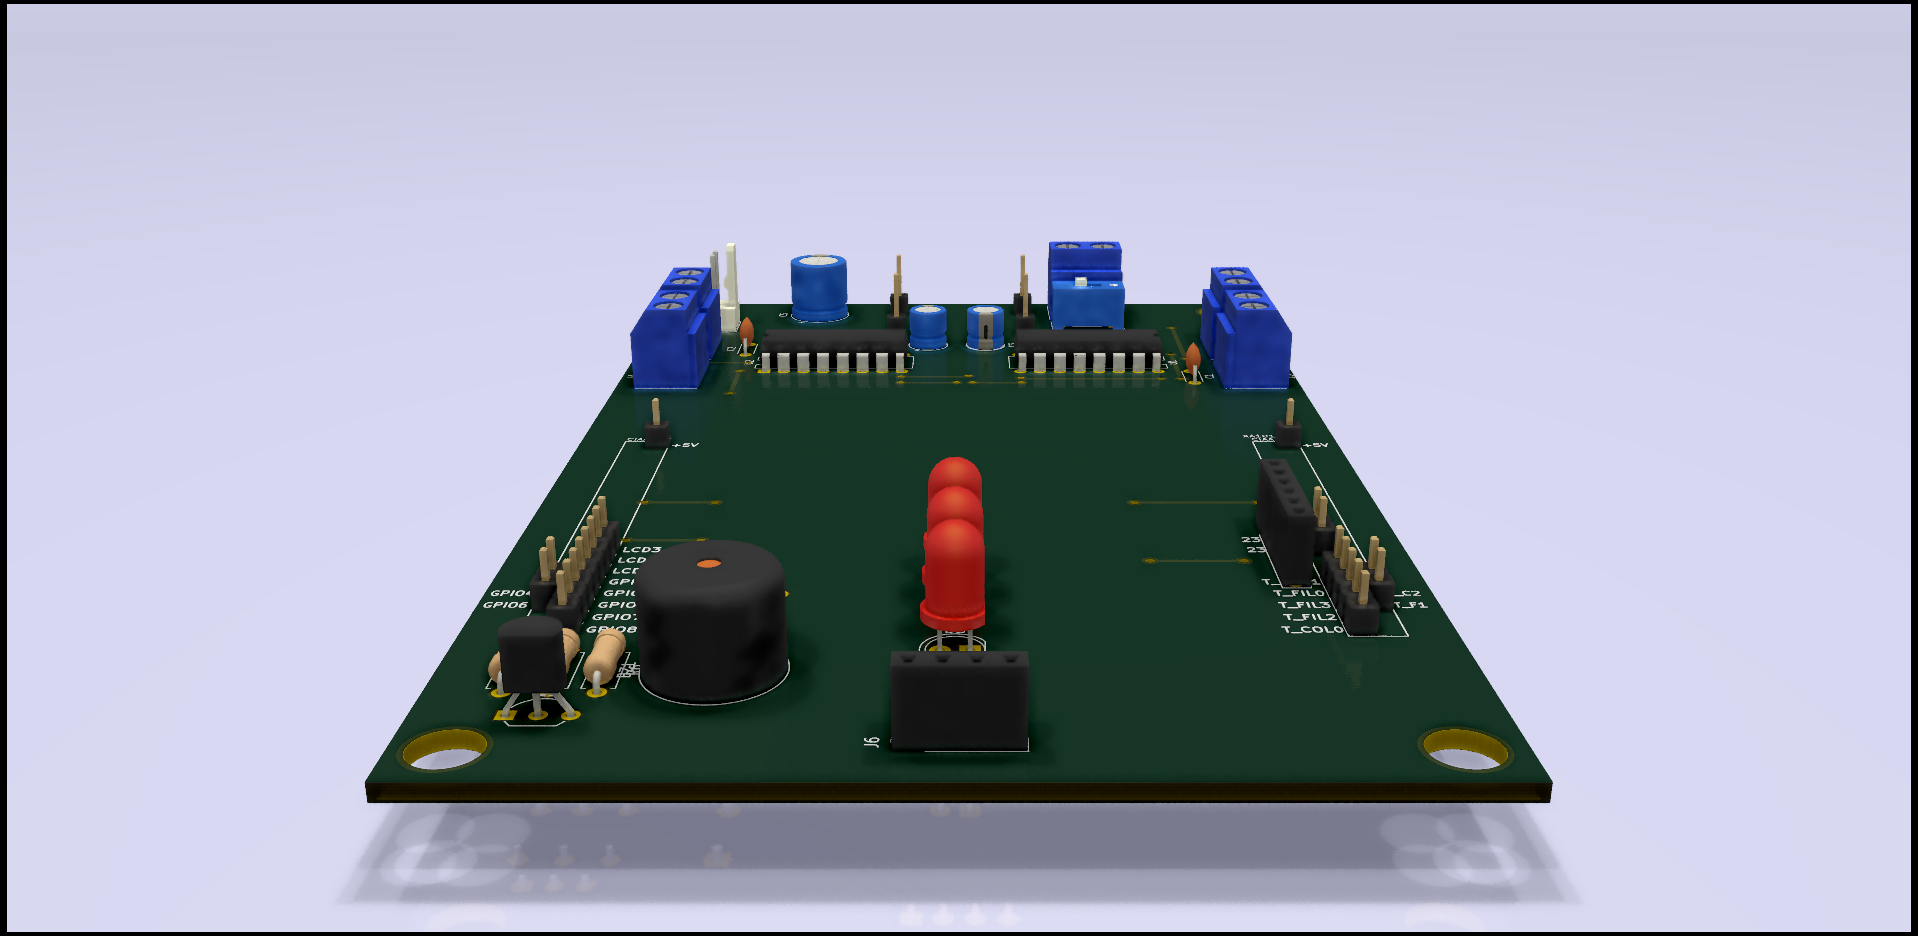
\includegraphics[width=0.5\linewidth]{informe_3/vista_frontal.png}} &
		\subfloat[Superior]{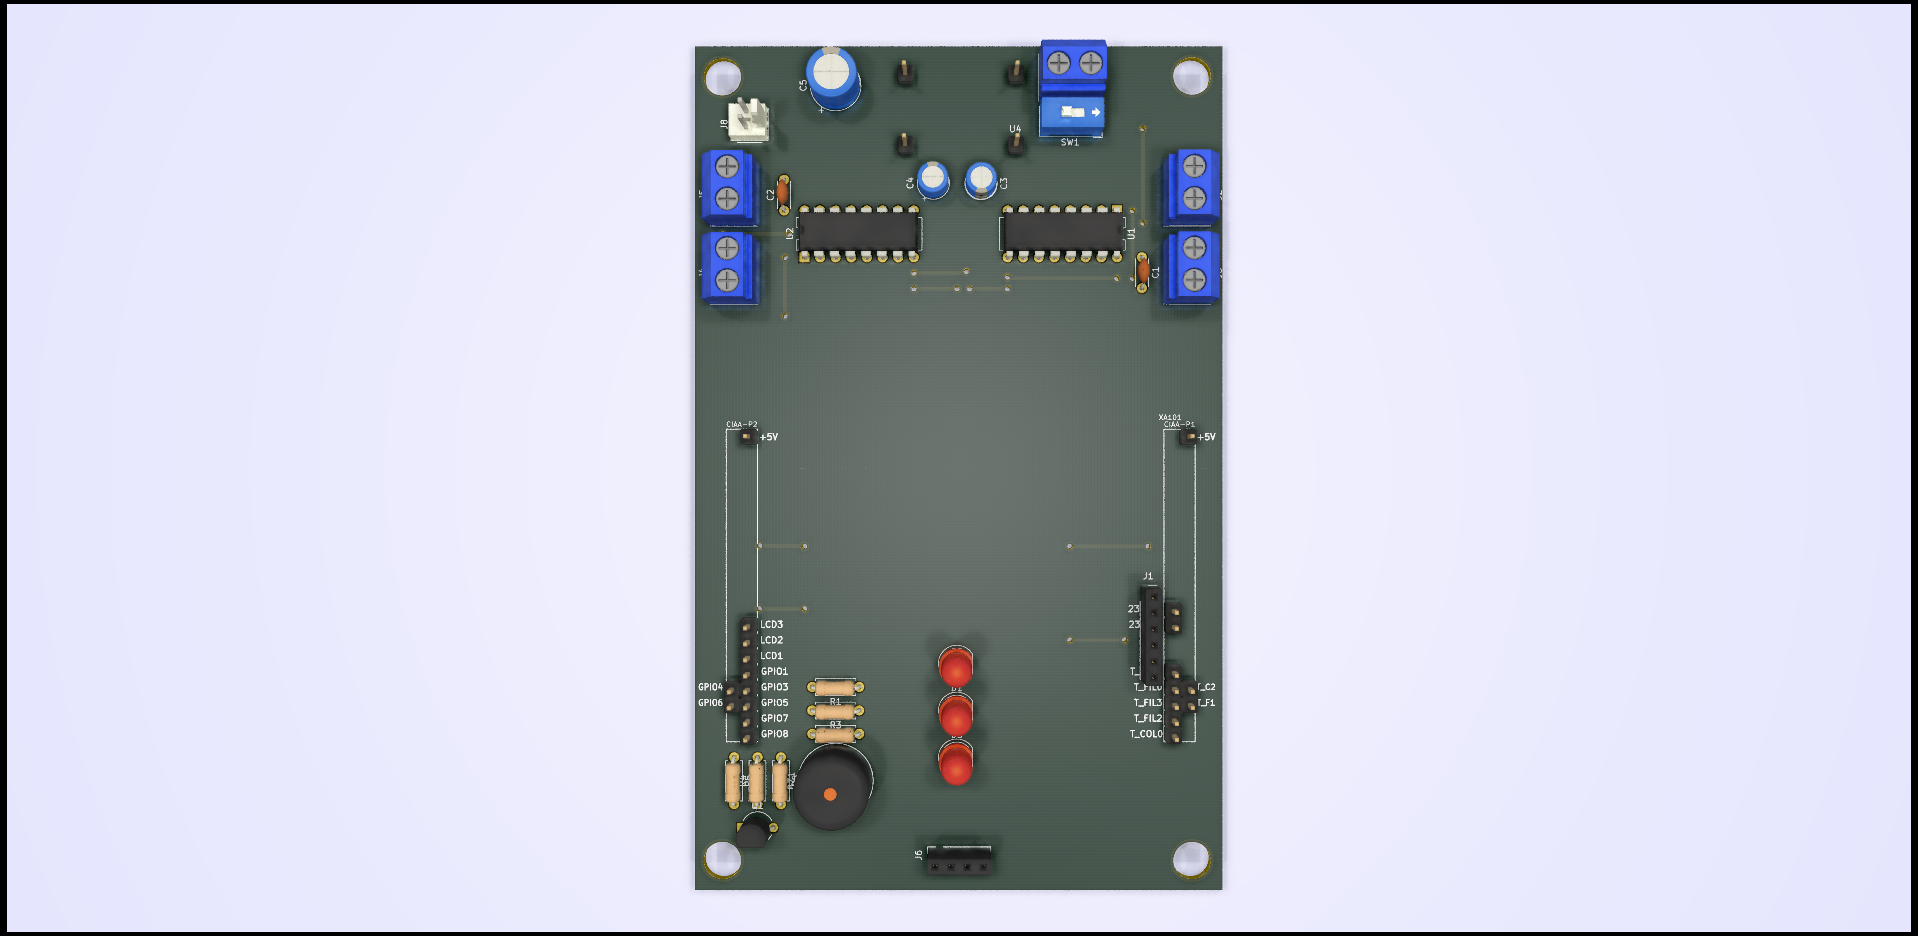
\includegraphics[width=0.5\linewidth]{informe_3/vista_superior.png}} \\
		\subfloat[Izquierda]{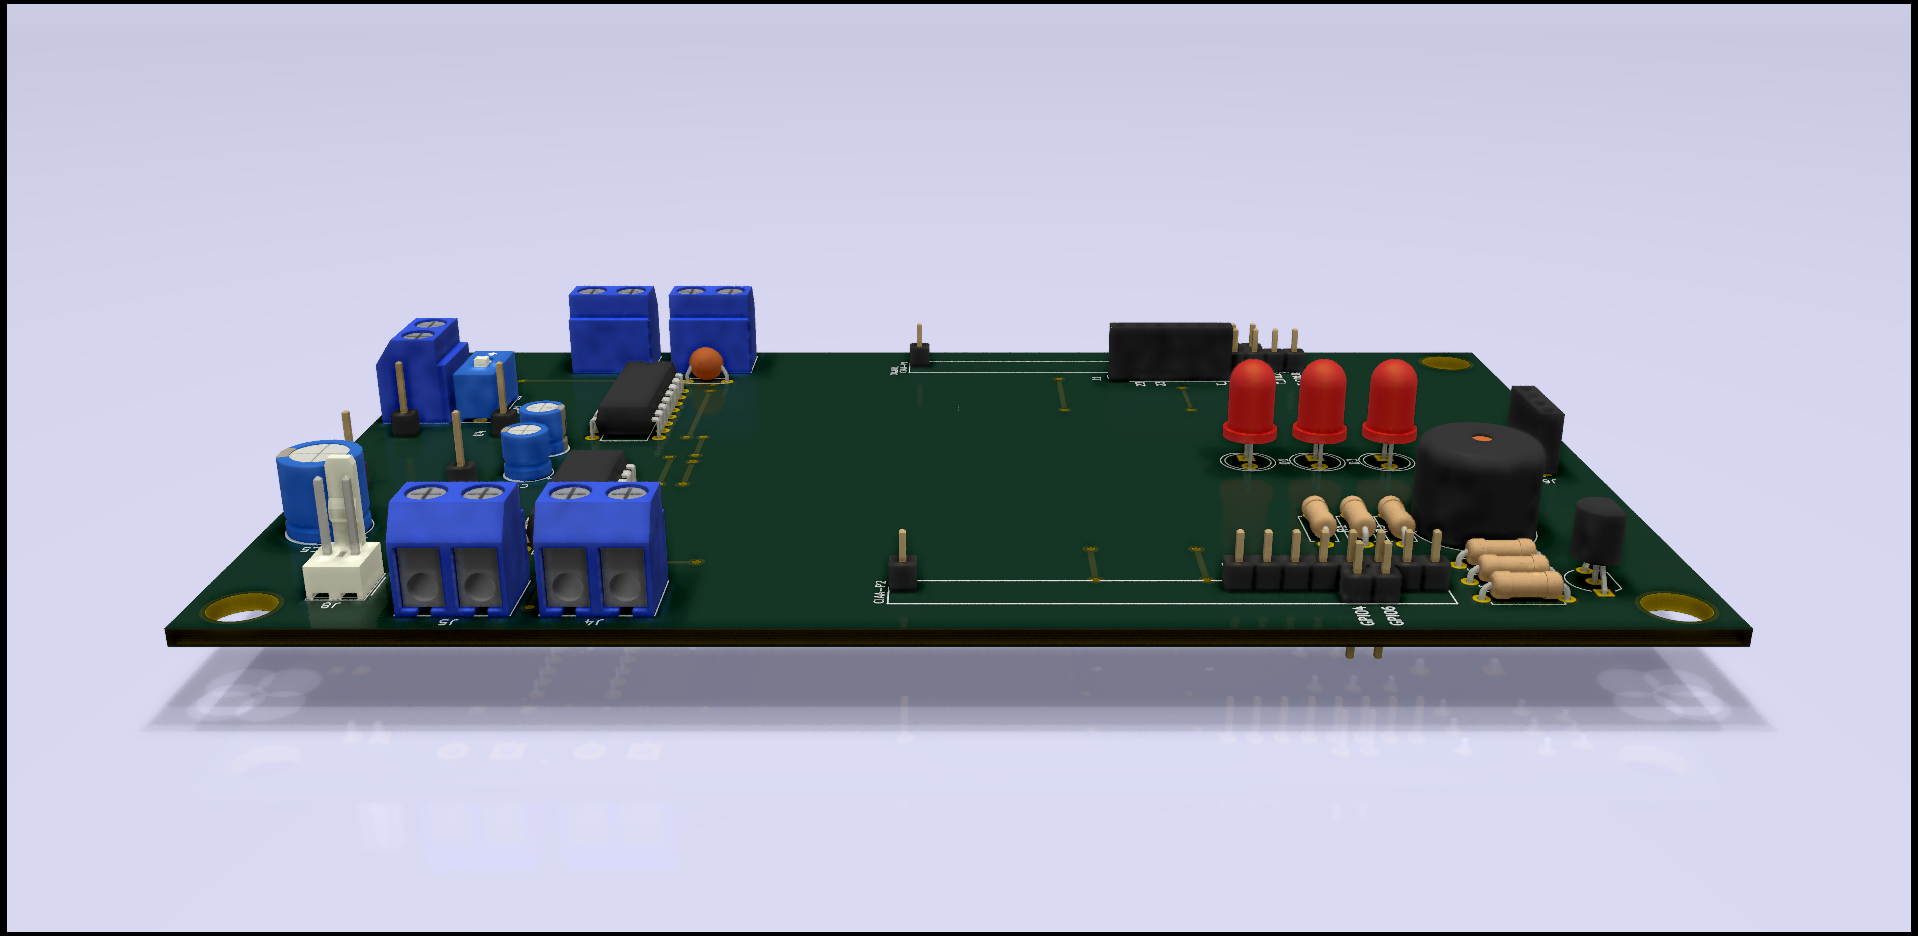
\includegraphics[width=0.5\linewidth]{informe_3/vista_lat_izq.png}} &
		\subfloat[Derecha]{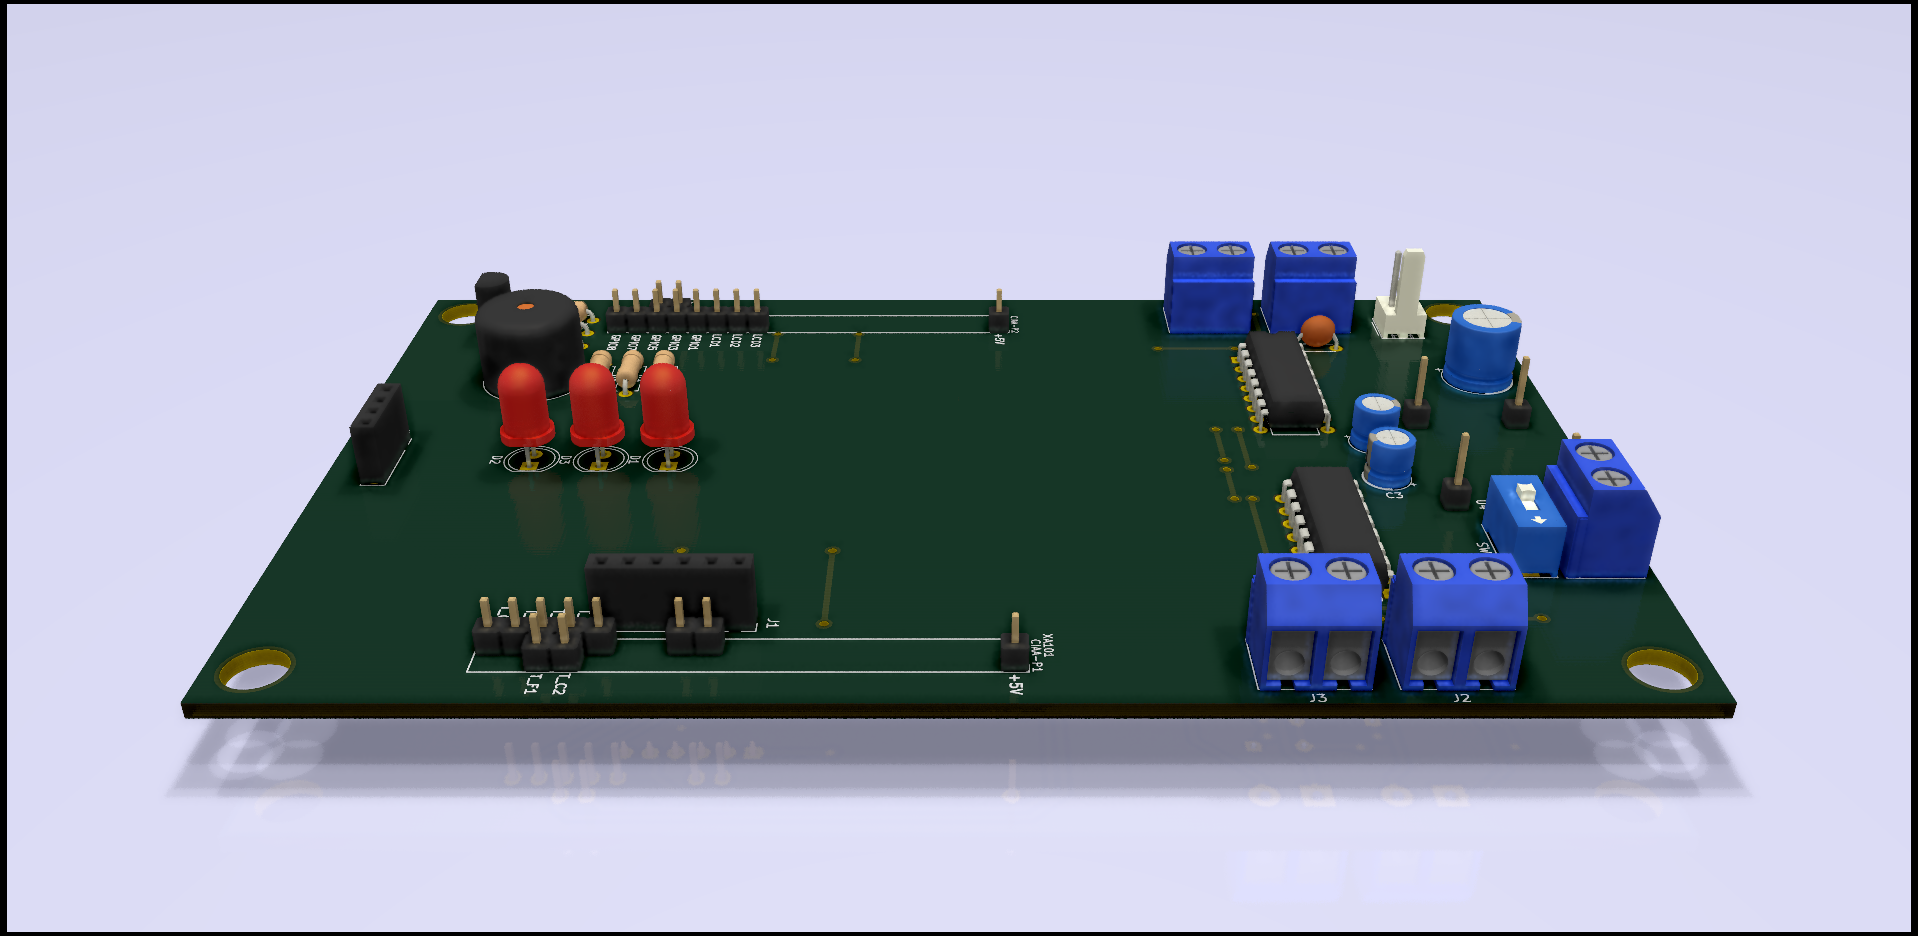
\includegraphics[width=0.5\linewidth]{informe_3/vista_lat_der.png}} 
	\end{tabular}
\caption{Renders generados en 3D con KiCAD}
\end{figure}


\section{Información general}

\begin{itemize}
	\item
	\textbf{HM-10} \url{https://github.com/ciaa/firmware\_v3/blob/master/examples/c/sapi/bluetooth/hm10\_uart\_bridge/EDU-CIAA-NXP\%20y\%20BLE\%204.0\%20HM10.pdf}
\end{itemize}

\section{Aplicaciones Externas}

\begin{itemize}
	\item
	\textbf{BLEJoystick} \url{https://play.google.com/store/apps/details?id=iyok.com.blejoystick}
\end{itemize}

\section{Datasheets}

\begin{itemize}
	\item
	\textbf{Transistor 2n7000} Disponible:
	\url{https://www.onsemi.com/pub/Collateral/2N7000-D.PDF}
	\item
	\textbf{L293D Texas } Disponible:
	\url{http://www.ti.com/lit/ds/symlink/l293.pdf}
	\item
	\textbf{L293D STMicroelectronics} Disponible:
	\url{https://www.st.com/resource/en/datasheet/l293d.pdf}
	\item 
	\textbf{HC-SR04} \url{http://raspoid.com/download/datasheet/HCSR04}
	\item 
	\textbf{HC-SR04} \url{https://cdn.sparkfun.com/datasheets/Sensors/Proximity/HCSR04.pdf4}
	\item 
	\textbf{HC-SR04} \url{https://www.electroschematics.com/hc-sr04-datasheet/}
\end{itemize}

\section{BOM}

\begin{longtable}[]{|c|c|p{9.5cm}|}
	\toprule
	Referencia & Encapsulado & Huella \tabularnewline
	\midrule
	\endhead
	
	BZ1 & - & Buzzer\_Beeper:Buzzer\_12x9.5RM7.6\tabularnewline
	C1 & C. Cerámico & Capacitor\_THT:C\_Disc\_D4.3mm\_W1.9mm\_ P5.00mm\tabularnewline
	C2 & C. Cerámico & Capacitor\_THT:C\_Disc\_D4.3mm\_W1.9mm\_ P5.00mm\tabularnewline
	C3 & C. Electrolítico &Capacitor\_THT:CP\_Radial\_D5.0mm\_P2.50mm\tabularnewline
	C4 & C. Electrolítico &Capacitor\_THT:CP\_Radial\_D5.0mm\_P2.50mm\tabularnewline
	C5 & C. Electrolítico &Capacitor\_THT:CP\_Radial\_D5.0mm\_P2.50mm\tabularnewline
	D1 & - & LED\_THT:LED\_D5.0mm\tabularnewline
	D2 & - & LED\_THT:LED\_D5.0mm\tabularnewline
	D3 & - & LED\_THT:LED\_D5.0mm\tabularnewline
	J1 & - & Connector\_PinSocket\_2.54mm:PinSocket\_1x06\_ P2.54mm\_Vertical\tabularnewline
	J2 & - & TerminalBlock:TerminalBlock\_bornier-2\_P5.08mm\tabularnewline
	J3 & - & TerminalBlock:TerminalBlock\_bornier-2\_P5.08mm\tabularnewline
	J4 & - & TerminalBlock:TerminalBlock\_bornier-2\_P5.08mm\tabularnewline
	J5 & - & TerminalBlock:TerminalBlock\_bornier-2\_P5.08mm\tabularnewline
	J6 & - & Connector\_PinSocket\_2.54mm:PinSocket\_1x04\_ P2.54mm\_Vertical\tabularnewline
	J7 & - & TerminalBlock:TerminalBlock\_bornier-2\_P5.08mm\tabularnewline
	J8 & KK254 & Connector\_Molex:Molex\_KK-254\_AE-6410-02A\_1x02\_P2.54mm\_Vertical\tabularnewline
	Q1 & TO-92 & Package\_TO\_SOT\_THT:TO-92\_Inline\_Wide\tabularnewline
	R1 & DIN0207 & Resistor\_THT:R\_Axial\_DIN0207\_L6.3mm\_D2.5mm\_ P7.62mm\_Horizontal\tabularnewline
	R2 & DIN0207 & Resistor\_THT:R\_Axial\_DIN0207\_L6.3mm\_D2.5mm\_ P7.62mm\_Horizontal\tabularnewline
	R3 & DIN0207 & Resistor\_THT:R\_Axial\_DIN0207\_L6.3mm\_D2.5mm\_ P7.62mm\_Horizontal\tabularnewline
	R4 & DIN0207 & Resistor\_THT:R\_Axial\_DIN0207\_L6.3mm\_D2.5mm\_ P7.62mm\_Horizontal\tabularnewline
	R5 & DIN0207 & Resistor\_THT:R\_Axial\_DIN0207\_L6.3mm\_D2.5mm\_ P7.62mm\_Horizontal\tabularnewline
	R6 & DIN0207 & Resistor\_THT:R\_Axial\_DIN0207\_L6.3mm\_D2.5mm\_ P7.62mm\_Horizontal\tabularnewline
	SW1 & - & Button\_Switch\_THT:SW\_DIP\_SPSTx01\_ Slide\_9.78x4.72mm\_W7.62mm\_P2.54mm\tabularnewline
	U1 & DIP16 & Package\_DIP:DIP-16\_W7.62mm\tabularnewline
	U2 & DIP16 & Package\_DIP:DIP-16\_W7.62mm\tabularnewline
	
	\bottomrule
\end{longtable}

\section{Imágenes de los Componentes}

\subsection{mini360}

\begin{figure}[H]
	\centering
	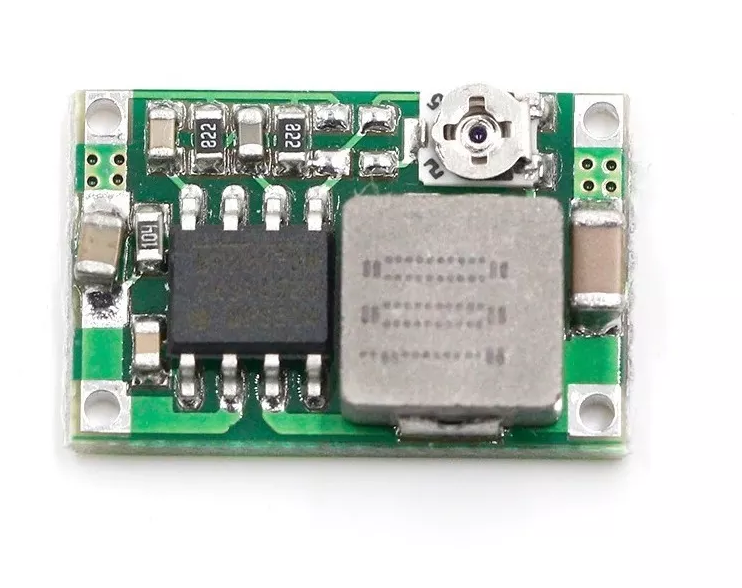
\includegraphics[width=0.4\textheight, angle=90]{informe_3/mini360.png}
	\caption{Fuente Step-Down}
	\label{fig:step-down}
\end{figure}